\documentclass{article}

\usepackage[margin=0.7in]{geometry}
\usepackage{amsmath,amssymb}
\usepackage{graphicx}
\usepackage{float}

\title{Electromagnetics}
\author{Emmanuel Estallo}


\begin{document}
\maketitle 
 
\section{Electric Fields}
\noindent 
The electric force between two point charges are obtained by 
$$\vec{F} = \frac{1}{4\pi\epsilon_0}\frac{Q_1 Q_2}{R^2}$$
If the charges are similar in polarity, then $\vec{F}> 0$. Otherwise, 
$\vec{F} < 0$.
Similarly, the electric field intensity can be obtained by placing a test charge $Q_t$ 
at any point and obtaining the net force that is experienced by the charge at that point.
$$\vec{E} = \frac{\vec{F_t}}{Q_t}$$

\subsection{Fields from Continuous Charge Distributions}
The volume charge density is denoted by $\rho_v$. The amount of charge stored in 
in a small volume $\Delta{v}$ is then $$\Delta{Q} = \rho_v \Delta{v}$$ and $\rho_v$
is mathematically defined as $$\rho_v = \lim_{\Delta{v}\to 0} 
\frac{\Delta{Q}}{\Delta{v}}$$ The total charge is then obtained by 
$$Q = \int_{vol} \rho_v dv$$

\subsection{Fields from Infinite Charge Distributions}
\subsubsection{Field of a Line Charge}
\noindent 
Consider a line charge with an infinite length extending from the negative z axis 
to the positive z axis. Varying $\vec{a_z}$ does not change the 
experienced electric field since it has an infinite length. So does changing 
$\vec{a_\phi}$ with a constant $\vec{a_\rho}$. The only thing that affects the
electric field magnitude is $\vec{a_\rho}$ 

\begin{figure}[H]
    \center
    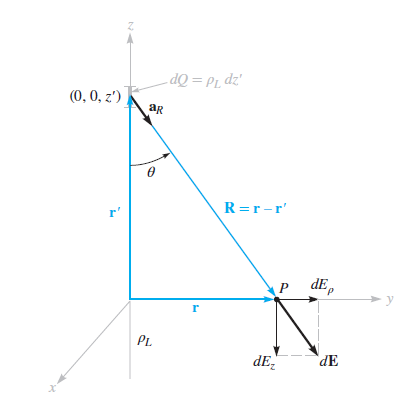
\includegraphics[scale=0.5]{inf_line_charge}
\end{figure}

\noindent
Here, we select an arbitrary point along the y axis $P(0,y,0)$.
\newpage 
\noindent 
Consider an infinitesimal charge $dQ$ from a slice of the line charge with length $z'$.
Now, $$dE = \frac{1}{4\pi\epsilon_0}\frac{\rho_L dz'}{\vec{R}^2}$$ where $\rho_L$ is
the linear charge density.
\vspace{8pt}
\\ Note that here, $\vec{R} = \vec{r} - \vec{r'}$ where $\vec{r} = y\vec{a_y} = 
\rho\vec{a_\rho}$ and $\vec{r'} = z'\vec{a_z}$. Thus, 
\begin{align*}
dE &= \frac{1}{4\pi\epsilon_0} \frac{\rho_L dz' (\rho\vec{a_\rho} - z'\vec{a_z})}
{|(\rho\vec{a_\rho} - z'\vec{a_z})|^3} \\
&= \frac{1}{4\pi\epsilon_0}\frac{\rho_L dz' (\rho\vec{a_\rho} - z'\vec{a_z})}
{(\rho^2 + z'^2)^\frac{3}{2}}
\end{align*}
Since varying $z'$ does not affect the electric field magnitude, 
\begin{align*}
\vec{dE} &= \frac{1}{4\pi\epsilon_0}\frac{\rho_L dz' \rho\vec{a_\rho}}
{(\rho^2 + z'^2)^\frac{3}{2}}\\
\vec{E} &= \int_{-\infty}^{\infty}\frac{1}{4\pi\epsilon_0}\frac{\rho_L dz' \rho\vec{a_\rho}}
{(\rho^2 + z'^2)^\frac{3}{2}}\\
&= \frac{1}{4\pi\epsilon_0} \int_{-\infty}^{\infty}\frac{\rho_L dz' \rho\vec{a_\rho}}
{(\rho^2 + z'^2)^\frac{3}{2}}\\
&= \frac{\rho_L}{4\pi\epsilon_0} \int_{-\infty}^{\infty}\frac{dz' \rho\vec{a_\rho}}
{(\rho^2 + z'^2)^\frac{3}{2}}
\end{align*}
Using trigonometric substitution with $z' =\rho \tan\theta$,
\begin{align*}
\vec{E} &= \frac{\rho_L}{4\pi\epsilon_0} \int_{-\infty}^{\infty}\frac{dz' \rho\vec{a_\rho}}
{(\rho^2 + z'^2)^\frac{3}{2}}\\
&= \frac{\rho_L}{4\pi\epsilon_0} \int_{-\infty}^{\infty}\frac{dz' \rho\vec{a_\rho}}
{[\rho^2(1+\tan^2\theta)]^\frac{3}{2}}\\
&= \frac{\rho_L}{4\pi\epsilon_0} \int_{-\infty}^{\infty}\frac{dz' \rho\vec{a_\rho}}
{[\rho^2(1+\tan^2\theta)]^\frac{3}{2}}\\
&= \frac{\rho_L}{4\pi\epsilon_0} \int_{-\infty}^{\infty}\frac{dz' \rho\vec{a_\rho}}
{\rho^3 \sec^3\theta}\\
&= \frac{\rho_L}{4\pi\epsilon_0} \int\frac{\rho\vec{a_\rho}}
{\rho^3 \sec^3\theta}\rho\sec^2\theta d\theta\\
&= \frac{\rho_L}{4\pi\epsilon_0} \int\frac{\rho\vec{a_\rho}}
{\rho^2 \sec\theta}d\theta \\
&= \frac{\rho_L}{4\pi\epsilon_0}\frac{\vec{a_\rho}}{\rho}\int
\cos\theta d\theta \\
&= \frac{\rho_L}{4\pi\epsilon_0}\frac{\vec{a_\rho}}{\rho}\sin\theta
\end{align*}
\noindent 
And,
\begin{equation*}
\vec{E}= \frac{\rho_L}{4\pi\epsilon_0}\frac{\vec{a_\rho}}{\rho}\frac{z'}{\sqrt{
    z'^2+\rho^2}} \Bigg|_{z=-\infty}^{\infty}
\end{equation*}
Finally,
$$ \boxed{\vec{E} = \frac{\rho_L}{2\pi\epsilon_0\rho}\vec{a_\rho}}$$
We can see that only the distance $\rho$ affects the magnitude. 

\newpage 
\subsubsection{Field of a Sheet of Charge}
Consider the sheet of charge placed at the y-z plane shown below. 
\begin{figure}[H]
    \center
    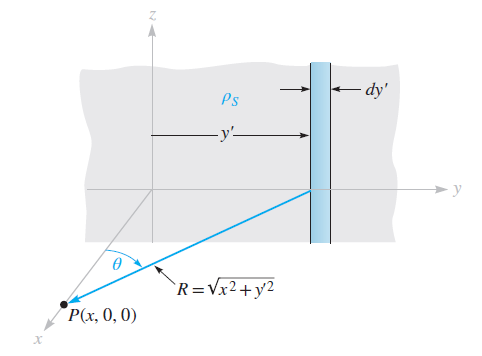
\includegraphics[scale=0.55]{inf_sheet_charge}
\end{figure}
\noindent 
We can use the electric field magnitude of a line charge to obtain the magnitude of 
this sheet. 
\vspace{8pt}
\\ We know that for a line charge, 
\begin{equation*}
\vec{E} = \frac{\rho_L}{2\pi\epsilon_0\rho}\vec{a_\rho}
\end{equation*}
Let $\rho_S$ be the surface charge density and $\rho_L = \rho_S dy'$ where $dy'$ is the 
infinitesimal width of the strip. We select an arbitrary point along the x axis.   
\begin{align*}
\vec{dE} &= \frac{\rho_S dy'\vec{a_N}}{2\pi\epsilon_0\sqrt{x^2+y'^2}}\cos\theta \\
&= \frac{\rho_S dy'\vec{a_N}}{2\pi\epsilon_0\sqrt{x^2+y'^2}}\frac{x}{\sqrt{x^2+y'^2}} \\
\vec{E}&=\int_{-\infty}^{\infty}\frac{\rho_S \vec{a_N}}{2\pi\epsilon_0}\frac{xdy'}
{x^2+y'^2} \\
&= \frac{\rho_S \vec{a_N}}{2\pi\epsilon_0} \int_{-\infty}^{\infty} \frac{xdy'}
{x^2+y'^2}\\
&= \frac{\rho_S \vec{a_N}}{2\pi\epsilon_0} \int_{-\infty}^{\infty} x
\frac{dy'}{x^2+y'^2}\\
&= \frac{\rho_S \vec{a_N}}{2\pi\epsilon_0}\tan^{-1}\left(\frac{y'}{x}\right)
\Bigg|_{y'=-\infty}^{\infty}
\end{align*}
Finally,
$$\boxed{\vec{E}=\frac{\rho_S}{2\epsilon_0}\vec{a_N}}$$
This means that the electric field magnitude from a sheet of charge is constant.
We can determine the sign depending on the normal vector from the sheet. 

\newpage 
\section{Flux Density, Gauss' Law, and Divergence}
\noindent 













\end{document}